
\documentclass{svmult}

\usepackage{makeidx}   % allows index generation
\usepackage{graphicx}  % LaTeX graphics tool for including eps-figure files
\usepackage{subeqnar}  % subnumbers individual equations within an array
\usepackage{multicol}  % used for the two-column index
\usepackage{physprbb}  % modified textarea for proceedings,lecture notes, etc.

                       % when manuscript is printed from paper, not from data
\makeindex             % used for the subject index
                       % please use the style sprmidx.sty with
                       % your makeindex program

\usepackage{axodraw}   % Feynman graphs


\newcommand{\greeksym}[1]{{\usefont{U}{psy}{m}{n}#1}}
\newcommand{\umu}{\mbox{\greeksym{m}}}
\newcommand{\udelta}{\mbox{\greeksym{d}}}
\newcommand{\uDelta}{\mbox{\greeksym{D}}}
\newcommand{\uPi}{\mbox{\greeksym{P}}}
\newcommand{\be}{\begin{equation}}
\newcommand{\ee}{\end{equation}}
\newcommand{\bea}{\begin{eqnarray}}
\newcommand{\eea}{\end{eqnarray}}
\newcommand{\bsa}{\begin{subeqnarray}}
\newcommand{\esa}{\end{subeqnarray}}
\newcommand{\eps}{\varepsilon}
\newcommand{\Veff}%
{{\cal V}^{\mbox{\scriptsize p}}_{\mbox{\scriptsize eff}}}
\newcommand{\Afr}{A^{\mbox{\scriptsize fr}}}
\newcommand{\Bfr}{B^{\mbox{\scriptsize fr}}}
\newcommand{\inn}{\mbox{\scriptsize in}}
\newcommand{\exx}{\mbox{\scriptsize ex}}
\newcommand{\Fs}{\mbox{\scriptsize F}}
\def\ra{\rightarrow}
\def\de{\Delta}
\def\al{\alpha}
\def\sig{\Sigma}
\def\gam{\Gamma}
\def\om{\omega}
\def\fdag{F^\dagger}
\def\ann{a_{nn}}
\def\kv{\vec{k}}
\def\epsk{\epsilon(\kv)}
\def\ll{\big\langle}
\def\rr{\big\rangle}
\def\sd{^3\!S\!D_1}
\def\pf{^3\!P\!F_2}
\def\ss{^1\!S_0}

\begin{document}

\title*{Enclosure (c): Dr.Scient Thesis project: Superfluidity and superconductivity in neutron stars and nuclear matter}

\author{Elise Bergli}

\institute{Department of Physics, University of Oslo} 

\maketitle  



\section{Introduction}

The main aim of 
this thesis project is a proper 
quantum-mechanical 
many-body treatment of pairing, superfluidity and superconductivity
in infinite nuclear matter, with possible ramifications to studies
of quantum liquids such as $^3$He and $^4$He 
and problems in solid state physics.

Pairing, superfluidity and superconductivity  lie
at the heart of many phenomena in solid state physics, quantum liquids, 
nuclear physics and the quantum
many-body problem in general. 
In infinitely extended nuclear systems such as neutron star matter 
and nuclear matter, 
the study of superfluidity, superconductivity and pairing has a 
long history predating the 1967 discovery of pulsars, 
which were soon identified as rapidly rotating magnetic neutron 
stars.  Interest in nucleonic pairing has intensified 
in recent years, owing primarily to experimental developments on two 
different fronts.  In the field of astrophysics, a series of $X$-ray 
satellites (including Einstein, EXOSAT, ROSAT, and ASCA) has brought a 
flow of data on thermal emission from neutron stars, comprising both upper 
limits and actual flux measurements.  The recent launching of the 
Chandra $X$-ray observatory provides further impetus for more incisive 
theoretical investigations.  On the terrestrial 
front, the expanding capabilities of radioactive-beam and heavy-ion 
facilities have stimulated a concerted exploration of exotic nuclei and 
nuclei far from stability, with special focus on neutron-rich species. 
Pairing plays a prominent role in modeling 
the structure and behavior of these new nuclei.  

The presence of neutron superfluidity in 
the crust and the inner part 
of neutron stars 
are thus considered well established 
in the physics of these compact stellar objects. 
To a first approximation, a neutron star 
is described as a neutral system of nucleons (and possibly heavier baryons) 
and electrons (and possibly muons) in beta equilibrium at zero temperature, 
with a central density several times the saturation density $\rho_0$ 
of symmetric nuclear matter. 
The gross structure of the star (mass, radius, pressure and density 
profiles) is determined by the Tolman-Oppenheimer-Volkov general 
relativistic equation of hydrostatic equilibrium, consistently with 
the continuity equation and the equation of state (which embodies the 
microscopic physics of the system).  The star contains (i) an {\it outer 
crust} made up of bare nuclei arranged in a lattice interpenetrated 
by relativistic electrons, (ii) an {\it inner crust} where a similar 
Coulomb lattice of neutron-rich nuclei is embedded in Fermi seas of 
relativistic electrons and neutrons, (iii) a {\it quantum fluid interior} 
of coexisting neutron, proton, and electron fluids, and finally 
(iv) a {\it core region} of uncertain constitution and phase (but 
possibly containing hyperons, a pion or kaon condensate and/or quark matter).

In the low density outer part of a neutron star, 
the neutron superfluidity is expected 
mainly in the attractive singlet $^1S_0$ channel. 
Qualitatively, this phenomenon can be understood
as follows.  At the relatively large average particle spacing at the 
``low'' densities involved in this region, i.e., $\rho \sim \rho_0/10$ 
with  $\rho_0$ the saturation density 
of symmetrical nuclear matter, 
the delocalized neutrons experience mainly the attractive component 
the $^1S_0$ interaction.   However, the pairing effect is quenched 
at higher densities, $\sim \rho_0$ and beyond, due to the strong 
short-range component of this interaction.  
At higher density, the nuclei in the crust dissolve, and one 
expects a region consisting of a quantum liquid of neutrons and 
protons in beta equilibrium. 
By similar reasoning, one 
expects thus $^1S_0$ proton pairing to occur in the quantum fluid interior, 
in a density regime where the proton contaminant (necessary for
charge balance and chemical equilibrium) reaches a partial 
density $\rho_p \sim \rho_0/10$. 
In this region, neutron superfluidity is expected to  
occur mainly in the coupled $^3P_2$-$^3F_2$ two-neutron channel. 
At such densities one may also expect superfluidity from 
other baryons such as e.g., 
hyperons to arise. The possibility for hyperon pairing is an entirely open
issue.
In the core of the star any superfluid 
phase should finally disappear, although the possibility of a
color superconducting phase opens up for interesting consequences.


Realistic {\it ab initio} prediction of the 
microscopic physics of nucleonic superfluid components in the interiors 
of neutron stars is crucial to a quantitative understanding of neutrino 
cooling mechanisms
that operate immediately after their birth 
in supernova events, as well as the magnetic properties, vortex structure, 
rotational dynamics, and pulse timing irregularities of these 
superdense stellar objects.  
In particular, when nucleonic species enter 
a superfluid state in one or another region of the star, suppression 
factors of the form $\exp (-\Delta_F /k_B T)$ are introduced 
into the expression for the emissivity, $\Delta_F$ being an appropriate 
average measure of the energy gap at the Fermi surface.  



A reliable estimate of the pairing gap can only be obtained through 
{\em ab initio} calculations, i.e., microscopic approaches using as input
realistic nucleon-nucleon interactions and summing large classes
of many-body correlations. 
In the many-body problem as applied to neutron star matter or quantum 
liquids, such a study has only partially been
performed. The crucial question deals with a correct and self-consistent 
treatment of 
so-called induced or screened interactions and the self-energy of the 
participant particles.

The size of the pairing gap in neutron star matter is still an unsettled 
problem. This means in turn that we cannot constrain properly the 
composition of matter in a neutron star. Moreover, even at low densities
the induced interaction plays a significant role. This has in turn
consequences for studies of weakly bound nuclei close to the 
stability line.

{\bf The aim of this thesis is thus to shed light on the renormalization
of the interaction in a nuclear medium, coupled with the solution
of the generalized gap equation.}
The formalism and numerical codes which are to  be developed will
have important consequences for our understanding of superfluidity
and superconductivity in other systems as well, ranging
from a proper treatment of the pairing gap above and below the
critical temperature to a description of pairing correlations in
dilute systems.


A detailed project description is given in the next section.

\section{Detailed project description}

\subsection{Green Function Formalism, Generalized Gap Equation}
\label{s:green}


The principal equations describing a superfluid system are the Gorkov
equations. These equations 
are a generalization of the Dyson equation 
for a normal Fermi system.
A diagrammatic representation of the Gorkov equations is shown in 
Fig.~\ref{f:gor}(a).
\begin{figure}[t] %------------------------------------------------------------
\includegraphics[height=.24\textheight,bb=10 600 10 830]{nsbk_gor.ps} %-20
\caption[]
{({\bf a}) Diagrammatic representation of the Gorkov equations.
 ({\bf b}) Equations for the self-energy $\sig$ and gap function $\de$}
\label{f:gor}
\end{figure} %-----------------------------------------------------------------
They express the relation between normal and anomalous propagators 
$G$ and $F$, defined by
\bsa
 G(1,2) &=& {1\over\I} \ll T(\Psi_1 \Psi_2^\dagger) \rr  \:,
\\
 F(1,2) &=& {1\over\I} \ll T(\Psi_1 \Psi_2) \rr  \:,
\esa
and the self-energy $\sig$ and gap function $\de$.
In a homogeneous system, these four quantitites depend only on a 
four-vector $k=(k_0,\kv)$ and can be written as $2\times 2$ matrices in 
spin space, for example,
\be
  {\bf\de}(k) = \left( \begin{array}{cc} 
  \de_{\uparrow\uparrow} & \de_{\uparrow\downarrow} \\ 
   \de_{\downarrow\uparrow} & \de_{\downarrow\downarrow} 
                    \end{array} \right)(k) \:.
\ee
Using the free fermion propagator
\be
  G_0(k) = { e^{\I 0 k_0} \over k_0 - \kv^2\!/2m + \mu + \I 0 k_0}  \:,
\ee
and defining
\be
 \eps(k) = {\kv^2 \over 2m} + \Sigma(k_0,\kv) - \mu  \:,
\ee
one can write the system of equations explicitly as
\be
  \left( \begin{array}{cc}
  [k_0 - \eps(+k)]{\bf 1}  & {{\bf\de}(k)}            \\ 
  {{\bf\de\!^\dagger}(k)}    & [k_0 + \eps(-k)]{\bf 1}
         \end{array} \right)
  \left( \begin{array}{c} {{\bf G}(k)} \\ {{\bf\fdag}(k)} \end{array} \right) =
  \left( \begin{array}{c} {\bf 1} \\ {\bf 0} \end{array} \right) \:, 
\label{e:fg}
\ee
where $\bf 1$ denotes the two-dimensional unit matrix.
In order to take into account at the same time pairing correlations 
$\de_S$ with spin $S=0$ and $S=1$, one can make the ansatz
\be
  {\bf\de} = \left( \begin{array}{cc} 
  0 & +\de_0 + \I \de_1 \\ 
  -\de_0 + \I \de_1 & 0
                    \end{array} \right) \:,
\ee
%${{\bf\fdag}}$ has the same structure, 
and equivalently for $\bf\fdag$,
whereas the self-energy $\bf\sig$ and $\bf G$ are diagonal in the spin indices.
If the ground state is assumed to be time-reversal invariant, the gap
function has in general the structure of a 
unitary triplet state,
i.e., it fulfills
\be
 {{\bf\de\!^\dagger}(k)} {\bf\de}(k) = \de(k)^2 \bf 1  \:,
\ee
where by $\Delta(k)^2$ we denote the determinant of ${\bf\de}$ in spin space. 

The system Eq.~(\ref{e:fg}) can then be inverted with the solution
\bsa
 G(k) &=& {k_0 + \eps(-k) \over D(k)} \:, 
\label{e:gg}
\\
 \fdag_S(k) &=& {\Delta_S(k) \over D(k)} \:,
\esa
where
\be
 D(k) = \left[ k_0 - \eps(+k) \right]  \left[ k_0 + \eps(-k) \right] 
         - \Delta_0(k)^2 - \Delta_1(k)^2  \:,
\label{e:dd}
\ee
that expresses the propagators $G$ and $\fdag$ in terms of $\sig$ and $\de$, 
respectively.

In order to determine uniquely the four quantities
one needs two more equations, 
which relate $\sig$ and $\de$ to the interaction.
These equations are displayed in Fig.~\ref{f:gor}(b) and read explicitly
\bsa
  \sig_{\al\al}(k) &=& {1\over\I} \int\! {{\rm d}^4 k' \over (2\pi)^4}
  \sum_\beta \ll k\al,k'\beta |T| k\al,k'\beta \rr  \, G_{\beta\beta}(k') \:,
\label{e:sga}
\\
  \de_{\al\beta}(k) &=& \,{\I} \int\! {{\rm d}^4 k' \over (2\pi)^4}
  \sum_{\al',\beta'} \ll k\al,-k\beta |\gam| k'\al',-k'\beta' \rr  
  \,F_{\al'\beta'}(k') \:,
\label{e:sgb}
\esa
where greek letters denote spin indices and
$T$ and $\gam$ are the scattering matrix
and the irreducible interaction kernel, respectively.
Clearly these equations cannot be solved in full generality, 
but one has to recur to some approximation at this stage.
The simplest, very common, BCS approximation, is to replace $T$ and $\Gamma$
by the leading term, namely the bare interaction $V$.
In this case the interaction is energy independent and the 
$k_0$ integration in Eqs.~(\ref{e:sga},\ref{e:sgb}) can be carried out 
trivially, leading to
\bsa
 \Sigma(\kv) &=& \sum_{\kv'} { v_{\kv'}^2 \over 2 } 
 %\ll \kv,\kv' |V| \kv,\kv' \rr_a    
 \Big[ \ll\kv,\kv'|{V_0+3V_1}|\kv,\kv'\rr 
\nonumber\\[-4mm]&&\hskip14mm 
 - \ll\kv,\kv'|{3V_1-V_0}|\kv',\kv\rr \Big] \,\;   
 \ ,\quad 
 v^2 = {1\over2}\left( 1 - {\eps\over E} \right) \:,
\\
 \Delta_S(\kv) &=& \sum_{\kv'} (u_S v)_{\kv'} 
 \ll \!\!+\!\kv',-\kv' |V_S| \!+\!\kv,-\kv \rr_a 
 \ ,\quad
 u_S v = {-\de_S\over 2E} \:,
\esa
where
\be
 E^2 = \eps^2 + \de_0^2  + \de_1^2  
 \ , \quad
 \eps = {\kv^2\over2m} + \sig(\kv) - \mu  \:.
\ee
Together with an equation fixing the chemical potential $\mu$ 
for given density $\rho$,
\be
 \rho = 2\sum_{\kv} v_{\kv}^2 \:,
\ee
this is the coupled set of equations that needs to be solved in order
to find the Hartree-Fock self-energy $\sig_{\rm HF}(\kv)$ and the 
BCS gap function $\de_{\rm BCS}(\kv)$ in a superfluid system.
In contrast to a normal Fermi system, the smooth occupation 
numbers $v_{\kv}^2$ instead of the Fermi function $\theta(k_F-|\kv|)$ 
appear in the HF equation.

\subsubsection{First goals}
The first part of this thesis is to solve the above Gorkov equations
with a simplified many-body approach to the bare interaction. This simplified
approach means that we are only summing particle-particle 
correlations, i.e., we are replacing the bare interaction with 
a so-called Brueckner $G$-matrix.
However, this has partly been done before in a partial wave approximation.
In this part of the thesis, we will solve the Gorkov equations
with the full angle-dependency of the $G$-matrix, that is
$\ll\kv, {\bf P} |G|\kv',{\bf P}\rr$ instead of its decomposition 
in partial waves, where $\kv$ is the relative momentum and
${\bf P}$ the center-of-mass momentum.
This means also that we will compute the Pauli operator, which prevents
scattering into occupied intermediate, without using the traditional
angle-average approximation.

This has never been done before, neither for pure neutron matter,
nor for asymmetric or symmetric nuclear matter. 
Avoiding  a partial wave approximation and an angle-averaged
Pauli operator, that is, keeping the full angle dependence of the 
interaction, will allow us to treat in a more direct way
the so-called induced interaction terms. 
This is important, since it is very difficult to compute the
Pauli operator for particle-hole intermediate states 
within the angle-averaging procedure.

The first part of the thesis leads to two explicit goals (these goals
may also lead to distinct publications):
\begin{enumerate} 
  \item Test the importance of the exact Pauli operator for the 
          energy per particle and effective interaction 
          in asymmetric nuclear matter and $\beta$-stable neutron star 
          matter 
          using various  Brueckner-Hartree-Fock approaches.
  \item Compute the pairing gap in symmetric, asymmetric nuclear matter 
        and $\beta$-stable neutron star 
          matter using the above effective interactions and single-particle
        energies within the BCS approximation. These results are in turn
        compared with the solution of the Gorkov equations with a full
        angle dependence.
\end{enumerate}


Fig.~\ref{f:gor} portrays  the relation between the pairing gap
$\Delta$, the self-energy $\Sigma$ and the propagators $G$ and $F$.
The crucial input to these equations is however the interaction $V$. 
The bare interaction $V$ is strongly changed in a many-body
system such as nuclear matter. How to compute such an in-medium
renormalized interaction
is highly non-trivial and 
leads us to the heart of this thesis and the next subsection, namely
how to renormalize in a self-consistent way the interaction vertex
$V$. This is an open problem with important consequences for several
fields in physics.


%==============================================================================
\subsection{A self-consistent renormalization of $V$}
\label{s:pol}

How to renormalize the bare interaction $V$ is an 
unsettled problem in many-body physics.
The influence of medium effects on pairing
constitutes an extremely difficult problem.
Consequently the results that can be found in the literature 
\cite{CHEN93,CLARK1,CHEN86,AINS89,WAMBACH,SCHU}
addressing this task in certain approximations agree only on the fact that
generally a strong reduction with respect to the BCS gap is obtained.
A collection of these results is displayed in Fig.~\ref{f:polgap}. 
It can be seen that the precise amount and density dependence of the 
suppression vary substantially between the different approaches 
and must be considered unknown for the time being. 
For pairing in the $^3P_2$ partial wave it is still an open question
whether the gap will be reduced or increased when polarization terms
are accounted for.
\begin{figure}[b] %------------------------------------------------------------
\includegraphics[height=.4\textheight,bb=40 380 40 690]{nsbk_pol.ps}
\caption[]
{The $\ss$ gap in pure neutron matter predicted in several publications
taking account of polarization effects.
The curve in the background shows the BCS result}
\label{f:polgap}
\end{figure} %-----------------------------------------------------------------

The first class of diagrams to be summed up are the so-called 
polarization diagrams to all orders in the 
particle-particle channel, but also including them in the particle-hole
channel, replacing the $T$-matrix by the general particle-hole
interaction $F$.
In this way a self-consistent scheme is established that is depicted 
in Fig.~\ref{f:pol}.
\begin{figure}[h] %------------------------------------------------------------
\includegraphics[height=0.45\textheight,bb=-0 410 -0 820]{nsbk_pic.ps}
\caption[]{
Determination of the interaction kernel $\Gamma$ in the gap equation ({\bf a}):
Polarization diagrams appear in the particle-particle channel ({\bf b}) 
as well as in the particle-hole channel ({\bf c}).
The leading diagrams in these channels   
are the bare potential $V$ (dashed line) and the $G$-matrix (double-dashed
line), respectively}
\label{f:pol}
\end{figure} %-----------------------------------------------------------------
It requires as input the Brueckner $G$-matrix and yields ideally the
interactions in the particle-particle as well as particle-hole channel,
$\Gamma$ and $F$, respectively.
The energy dependence 
of the full gap equation [see Eq.~(\ref{e:sgb})] needs to be 
taken into account.
This is obvious, since the interaction kernel becomes now a complex,
energy-dependent quantity.
To our knowledge, this problem has so far not been studied in detail 
in the literature. 
It is therefore not known how far the gap could be changed by this
more elaborate treatment of the equations.

Third, and in connection with the two previous points,
the choice of a particular interaction kernel 
requires also the choice of a compatible self-energy appearing in the 
gap equation.


This part of the project entails the development of a self-consistent
scheme for a renormalized interaction in the medium by summing
particle-particle, hole-hole and particle-hole diagrams to infinite order.
{\bf The equations for the interaction are coupled with the Gorkov equations
described in the previous subsection.}

This aim will be achieved through the following two steps (with several possible
publications)
\begin{enumerate}
 \item Using the full angle-dependence of an interaction which contains
       only particle-particle renormalizations such as the 
       Brueckner $G$-matrix, we start to compute 
       polarization effects using the  Babu-Brown induced interaction model 
       \cite{BABU,SJO73,BACK73,JACK82,DICK83,BACK85}. 
       The microscopic derivation 
       of this effective interaction starts from the following physical idea: 
       The particle-hole (p-h) interaction can be considered as made of a 
       {\em direct} component containing the short-range correlations and an 
       {\em induced} component due to the exchange of the collective excitations 
of the medium.
This approach serves two aims. First, it allows to gain insight into
the transformation of the interaction to the particle-hole channel. Secondly,
it offers a very physical interpretation of such corrections and can be compared 
with the more detailed calculations in the next step.
\item We then solve the full equations for the screening of particle-hole
corrections and renormalization of particle-particle and hole-hole
diagrams through the solution of 
the so-called Parquet equations \cite{JACK82,DICK83,mhj98}.
This will be our most complete effective interaction at the two-body 
level.
 \end{enumerate}
\section{Extension to other systems}
The formalism which will developed during this thesis
work has significant extensions to other physical systems.

It should suffice to mention studies of the superfluid transition
in dilute Fermi systems \cite{henning2000} as seen in 
spin-polarized Alkali gases \cite{stoof},
applications to quantum liquids
such as $^3$He \cite{glyde} or 
superconductivity in solid state physics as in seen in e.g., ultrasmall
metallic grains \cite{delft} or high $T_C$ superconductivity.

As a first extension, we plan to apply our formalism to studies
of superfluidity in quantum liquids
such as $^3$He.

\section{Working conditions}
The work will be done at  the theoretical 
nuclear physics group of the
Department of Physics, University of Oslo. This
group has a long-standing experience in many-body physics
and has worked intensively on neutron star physics during the 
last decade. At presently the group counts  three professors, 
two Phd students 
and 7 Msc students
working on various
apsects of many-body physics and nuclear physics. 
All necessary infrastucture will be provided
by the Department of Physics.
The group has extensive collaborations with the subatomic physics
group at the University of Bergen. 

A new national educational programme, which offers advanced graduate
courses on modern nuclear physics, has recently been established between
the groups in Bergen and Oslo. The aim is to provide a coherent and
upgraded nuclear physics curriculum in Norway.  

In addition, the theory activity in Oslo has extensive
international collaborations with several Universities and research 
laboratories in the USA, Europe and Japan. 
Eventual visits, for shorter
or longer periods, at foreign research institues
during the thesis work, form thus an important part of the 
present Phd programme.


\begin{thebibliography}{}
\addcontentsline{toc}{section}{References}


\bibitem{CHEN93}
 J. M. C. Chen, J. W. Clark, R. D. Dav\'e, and V. V. Khodel,
 Nucl. Phys. {\bf A555}, 59 (1993).
\bibitem{CLARK1} 
 J. W. Clark, C.-G. K\"allman, C.-H. Yang, and D. A. Chakkalakal,
 Phys. Lett. {\bf B61}, 331 (1976).
\bibitem{CHEN86} 
 J. M. C. Chen, J. W. Clark, E. Krotschek, and R. A. Smith,
 Nucl. Phys. {\bf A451}, 509 (1986).
\bibitem{AINS89} 
 T. L. Ainsworth, J. Wambach, and D. Pines,
 Phys. Lett. {\bf B222}, 173 (1989).
\bibitem{WAMBACH} 
 J. Wambach, T. L. Ainsworth, and D. Pines,
 Nucl. Phys. {\bf A555}, 128 (1993).
\bibitem{SCHU}  
 H.-J. Schulze, J. Cugnon, A. Lejeune, M. Baldo, and U. Lombardo,
 Phys. Lett. {\bf B375}, 1 (1996).

% Babu-Brown:
\bibitem{BABU} 
 S. Babu and G. E. Brown,
 Ann. Phys. (N.Y.) {\bf 78}, 1 (1973).
\bibitem{SJO73} 
 O. Sj\"oberg,
 Ann. Phys. (N.Y.) {\bf 78}, 39 (1973).
\bibitem{BACK73} 
 S.-O. B\"ackmann, C.-G. K\"allman, and O. Sj\"oberg,
 Phys. Lett. {\bf 43B}, 263 (1973).
\bibitem{JACK82} 
 A. D. Jackson, E. Krotschek, D. E. Meltzer, and R. A. Smith,
 Nucl. Phys. {\bf A386}, 125 (1982).
\bibitem{DICK83} 
 W. H. Dickhoff, A. Faessler, H. M\"uther, and Shi-Shu Wu,
 Nucl. Phys. {\bf A405}, 534 (1983).
\bibitem{BACK85} 
 S.-O. B\"ackmann, G. E. Brown, and J. A. Niskanen,
 Phys. Rep. {\bf 124}, 1 (1985).
\bibitem{mhj98} M.~Hjorth-Jensen, nucl-th/9811101 and in 
'Microscopic approaches to the structure of light nuclei, in 
Series on Advances in Quantum Many-Body Theory - Vol. 2
\bibitem{henning2000}H. Heiselberg {\em et al}, Phys. Rev. Lett. {\bf 85}, 2418 (2000). 
\bibitem{stoof}H. T. C. Stoof {\em et al}, Phys. Rev. Lett. {\bf 76}, 10 (1996).
\bibitem{glyde} Henry Glyde, Excitations in liquid and solid helium, 
(Oxford University Press, Oxford, 1994). 
\bibitem{delft} J. Von Delft and D.C. Ralph, Phys. Rep. {\bf 345}, 61 (2001).


% Self-energy:
\bibitem{BOZ}
 P. Bozek,
 Nucl. Phys. {\bf A657}, 187 (1999); Phys. Rev. {\bf C62}, 054316 (2000).

% Books: 
\bibitem{ABRI}
 A. A. Abrikosov, L. P. Gorkov, and I. E. Dzyaloshinskii,
 {\it Methods of Quantum Field Theory in Statistical Physics}
 (Prentice-Hall, Englewood Cliffs, 1963).
\bibitem{NOZ66} 
 P. Nozi\`{e}res, 
 {\em Theory of Interacting Fermi Systems}
 (Benjamin, New York, 1966).
\bibitem{SCHRIEF}
 J. R. Schrieffer, 
 {\it Theory of Superconductivity}
 (Addison-Wesley, New York, 1964).
\bibitem{MIG}
 A. B. Migdal, 
 {\it Theory of Finite Systems and Applications to Atomic Nuclei}
 (Benjamin, New York, 1964). 
\bibitem{RS} 
 P. Ring and P. Schuck,  
 {\em The Nuclear Many-Body Problem}
 (Springer, Berlin, 1980).
\bibitem{FW}
 A. L. Fetter and J. D. Walecka, 
 {\it Quantum Theory of Many-Particle Systems} 
 (McGraw-Hill, New-York, 1971).



\end{thebibliography}

\end{document}

